\documentclass{article}

\usepackage{graphicx}
\graphicspath{ {figures/} }

\usepackage{color}
\newcommand{\todo}[1]{{\color{red}{\textbf{\em [TODO: #1]}}}}

\title{A Practical Encryption Workshop}
\author{Marcella Hastings}
\date{}
\begin{document}
\maketitle

\section{What is encryption?}
I study computer security. I may have a different model of paranoia than others. But one of my goals
is to understand what is happening, what is feasible, and what is unlikely given the current state
of technology. The ability to distinguish a plausible threat from cyber posturing is an important
and empowering skill, but it can feel like an insurmountable task when there’s so much left to
learn about technology. The goal of this talk is to give you some background in a variety of
privacy technologies so that you can start to learn to make those decisions for yourself. We
also want to promote encryption everywhere, so hopefully by the end of the session you’ll be able
to install and use these tools.
\subsection{Threat modeling}
A necessary part of any security talk (any talk, really) is defining the context. In security, this
is called threat modeling. Basically, in order to evaluate whether a technology is secure, we need
to decide what it ought to be secure against. Who’s trying to break it? How powerful are they? What
devices and computers do they have access to? How much time do they have? Answering these questions
is an important step in contextualizing what kind of security you can get from any given tool, so
we’ll try to frame each topic with the threat model that’s behind it. 
Example: We want to build something to prevent people from stealing your food. What’s the
threat model? Suppose our attacker is a random person on the street. They do not have regular
access to your home without your permission. They don’t know where your refrigerator is. They don’t
know your schedule. Now suppose our attacker is your roommate. They have a key to your house.
They know where you keep your food. They know when you’re at school or work. Your defense
mechanisms against these two attackers are very different, and this is something you need to define
when you’re building your tools.
\subsection{Expectations}
This is where we’ll give some broad, sweeping expectations about what you can get out of
encryption.
The encryption ecosystem 

\section{Secure browsing}
\subsection{cookies/history (private browsing)}
A web browser is a product that allows you to access web pages (Chrome, IE, Safari, Firefox). Some
web pages are static; every time you access them, they are exactly the same. Others want to keep
some kind of state: who is logged in, what was your search query, what kinds of shoes have you
shopped for. Sometimes these are encoded in a url <example>. Other times, they are put in cookies
and stored in your browser. Whenever you return to a site that has stored a cookie in your
browser, it requests that information and uses it to personalize your site experience.
Sometimes this is great (staying logged in to facebook). Sometimes it’s vaguely creepy (stores
remember what items you were looking at three weeks ago). Sometimes it’s invasive and unwanted
(tracking preferences and habits to be sold to ad companies). These persistent cookies will be
stored by the browser until you delete them or until they reach their expiration date. 
Private browsing automatically deletes cookies when you close the browser. Prevents long-term
tracking. 
\subsection{HTTPS}
The internet works by encoding information (what a web page looks like, what your username is,
what comment you just typed in) into PACKETS
They contain (for simplicity’s sake) a sender, a receiver, and message contents. 
HTTP is the protocol/procedure for sending these packets from one computer to another. HTTPS
(secure HTTP, or HTTP with SSL (secure socket layer)) encrypts the contents of the message but the
participants are still visible

\begin{figure}
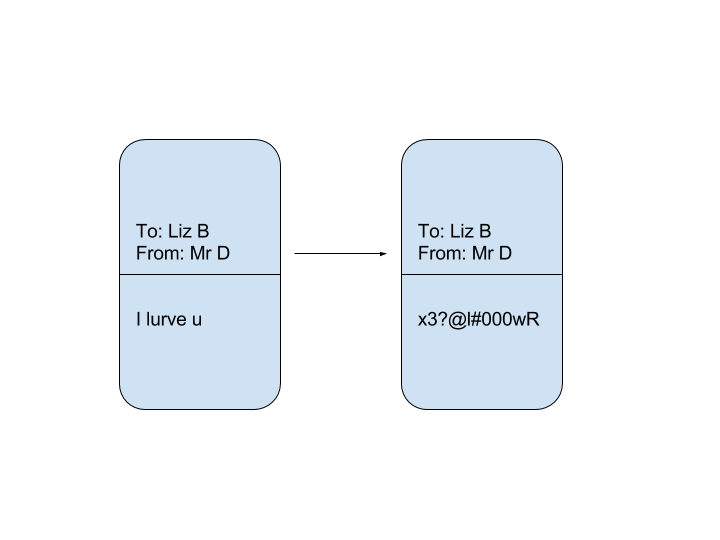
\includegraphics[width=\textwidth]{https}
\caption{What you get from HTTPS}
\end{figure}

\subsection{TOR}
If we recall HTTPS, we have packets with a receiver, a destination, and a message. HTTPs encrypts
the message. However, sometimes you may prefer to keep the participants private, or you may not
wish to disclose your identity to the server. This is not built-in functionality on the internet:
every packet must have a src/dest. The Tor protocol lets Alice choose 3 random computers on
the network and routes her packet through all three.  

\todo{get TOR graphic}

\subsection{VPNs}
Every time you connect to the internet, your request is sent through an internet service
provider. This means your ISP can see everything.
A VPN encrypts your traffic and sends it to a secure server first, and to its final destination
second. This means that your ISP can’t tell what you’re actually connecting to because all
your connections go to the VPN, and all of the content is encrypted. This can also protect you
from eavesdroppers on unsecured wifi networks (ie the coffeeshop).
Cons: slower connection, place trust in your VPN

\begin{figure}
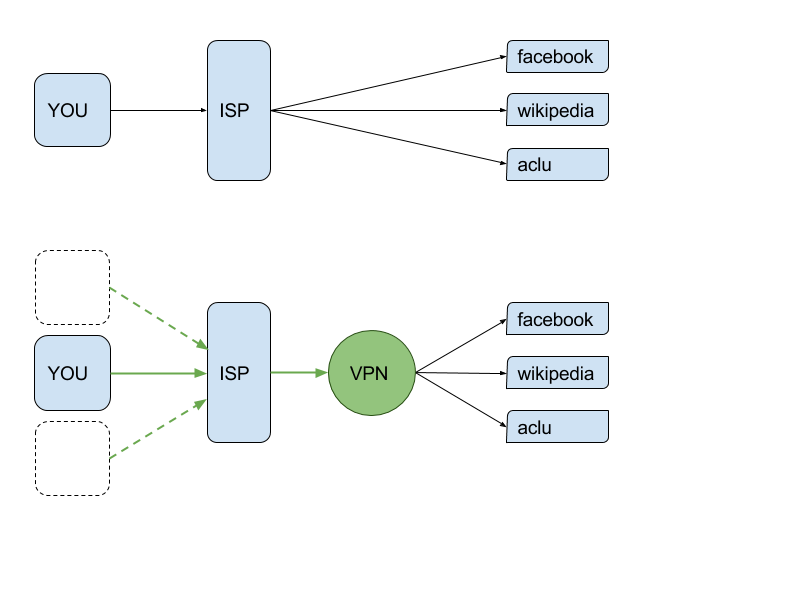
\includegraphics[width=\textwidth]{vpn}
\caption{This is approximately what VPNs do}
\end{figure}



\section{Secure messaging}
\subsection{whatsapp/messenger}
\subsection{Signal}

\section{Web services: what can companies do with your data}
\subsection{Backdoors} 
(i.e. can companies decrypt your data?)
\subsection{Subpoenas}
\subsection{Warrant canaries}



\end{document}
